\documentclass{article}

\title{ECE447 - Homework 3 - Q2 Revision}
\author{Chase Lotito - SIUC Undergraduate}
\date{}

%% PACKAGES %%

\usepackage{amsmath, amsfonts, amssymb, amsthm}
\usepackage{braket}
\usepackage{listings}
\usepackage{geometry}
\usepackage{xcolor}
\usepackage{textcomp}
\usepackage{graphicx}
\usepackage{fancyhdr}

%%%%%%%%%%%%%%

\graphicspath{{./images}}
\setlength\parindent{0pt}       % globally supress indentation

%% LISTINGS CONFIG %%

\definecolor{purple2}{RGB}{153,0,153} % there's actually no standard purple
\definecolor{green2}{RGB}{0,153,0} % a darker green

\lstset{
  language=Python,                   % the language
  basicstyle=\normalsize\ttfamily,   % size of the fonts for the code
  frame = single,
  % Color settings to match IDLE style
  keywordstyle=\color{orange},       % core keywords
  keywordstyle={[2]\color{purple2}}, % built-ins
  stringstyle=\color{green2},%
  showstringspaces=false,
  breaklines=true,
  numbers=left,
  commentstyle=\color{red},%
  upquote=true,                      % requires textcomp
}

\begin{document}

%%%%%%%%%%%%%%%%%%%%%
\pagestyle{fancy}

\maketitle

% attempt to make nice header
\fancyhead{}
\fancyhead[CH]{\normalsize{SOUTHERN ILLINOIS ECE / Chase Lotito / Spring 2024}}

%% THE HOMEWORK BEGINS HERE %%

From the last submission, the plot for the tunneling coefficient \(T\) was incorrect. Since \(T\) represents a probability, it must be between 0 and 1, which the previous plot did not reflect.

\section{Question 2}

Plot the tunneling probability, \(T\), as a function of electron energy, \(E\), for the conduction electron through a potential barrier of thickness 15 \AA ~ and a height equal to 0.3eV, with the electron effective mass of \(0.067m_0\). Vary \(E\) from 0 to 4eV in a step of 0.001eV. Replot the characteristic on the same graph when the barrier thickness is reduced to 5\AA. How can your finding explain the origin of excessive leakage currents as seen in modern nanoscale MOSFETs?

\subsection{Q2 Revisions}

The equation used to calculate the tunneling coefficient.

\begin{equation}\label{eq:tunnel}
    T = \left[ 1 + \frac{V^2_0 \sinh^2 (k_{II} W)}{4 E(V_0 - E)} \right]^{-1}
\end{equation}

\(V_0\) is the barrier height, \(W\) is the barrier width, \(E\) is the energy of the conduction band electron, and \(k_{II}\) is the wavenumber inside the potential barrier given by:

\begin{equation}\label{eq:k}
k_{II} = \frac{\sqrt{2  m^* (V_0 - E)}}{\hbar} 
\end{equation}

From Eq. \ref{eq:k}, we can only have real solutions for \(V_0 \geq E\). If \(V_0 = 0.3\)eV, then we should see \(T \to 1\) as \(E \to 0.3\)eV.


\subsubsection{The Code}

\begin{lstlisting}
# Chase Lotito - SIUC - ECE447 HW 3 - Q2: Tunneling Probability Graphs

# We wish to write a script that will plot the tunneling probability of an electron T as a function of the electron's energy E.

# We have a conduction electron with an effective mass of 0.067m, potential barrier thickness of 15A, and potential barrier height of 0.3eV

import matplotlib.pyplot as plt
import numpy as np
import math

# IMPORTANT CONSTANTS
q = 1.6e-19                 # fundamental charge / eV-to-J conversion factor
h = 6.63e-34                # Planck's constant [J*s]
hbar = h / ( 2 * math.pi )  # Reduced Planck's Constant
mfe = 9.8e-31               # mass of free electron
me = 0.067 * mfe            # effective mass of electron
a1 = 15e-10                 # potential barrier thickness
a2 = 5e-10                  # second potential barrier thickness
v0_eV = 0.3                 # potential barrier height in eV
v0_J = v0_eV * q            # potential barrier height in Joules

# Tunneling Probability Function
def tunnelProb(x, a):
    # Find the energy of the electron 
    energy = x * q       # making sure to convert eV to J
    k =  ( 2 * me * (v0_J - energy) )**0.5 / hbar  # second wavenumber
    
    # find numerator and denominator of fraction
    numerator = v0_J**2 * (np.sinh(k * a))**2 
    denominator = 4 * energy * (v0_J - energy)
    
    ans = 1 + (numerator / denominator)
    #return final answer (reciprocal)
    return (1 / ans)

# Ranges for graph
x = np.linspace(0,4,4000)     # Gives a range of 0 to 4 with steps of 0.001
y1 = tunnelProb(x, a1)        # Evals tunneling prob of 15A barrier thickness
y2 = tunnelProb(x, a2)        # Does this again with 5A barrier thickness

# Plot the graphs
plt.plot(x, y1, label = '15Å')
plt.plot(x, y2, label = '5Å')

# Find the maximums of the functions!
max_x = np.argmax(tunnelProb(x, a1))
max_y = tunnelProb(float(max_x), a1)
print(f"The maximum of the function occurs at x = {x[max_x]} with a value of {max_y}")

# Plot the maximums of our functions!
# plt.plot(max_x, 5e-6, marker="o", markersize=2, markeredgecolor="orange", markerfacecolor="orange")

# Console log some values for import debug
print('[15A] E = ' + '{:e}'.format(0.2 * q) + ', T = ' + '{:e}'.format(tunnelProb(0.2,a1)))
print('[5A] E = ' + '{:e}'.format(0.2 * q) + ', T = ' + '{:e}'.format(tunnelProb(0.2,a2)))

# Labels and Titles
plt.xlabel('Energy (eV)')
plt.ylabel('Tunneling Coefficient')
plt.title('Tunneling Coefficient for 5Å and 15Å Well')

# Axis formatting
plt.xlim(0,4)

# Show the plot
plt.legend()
plt.show()
\end{lstlisting}

\clearpage

\subsubsection{The Plot}
\begin{figure}[!ht] 
    \centering
    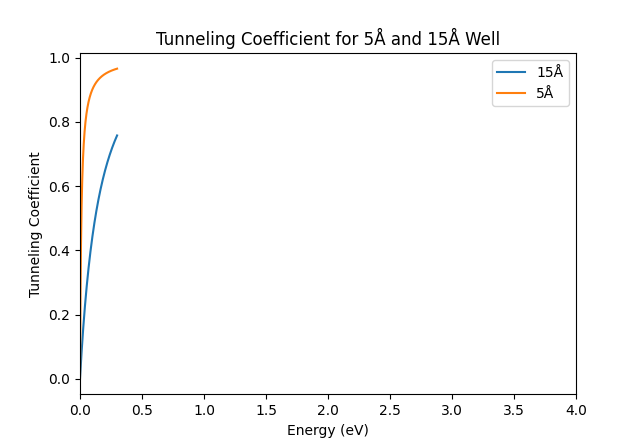
\includegraphics[width = 10cm]{plot2.png}
    \caption{Tunneling Coefficient w.r.t. Electron Energy}
\end{figure}

As the electron increases in energy, the electron's probability of tunneling through the potential barrier increases and approaches 1 (100\% chance of tuennling). Eq. \ref{eq:tunnel} is an approximation, so we don't see the two curves fully reach 100\% tunneling as they reach 0.3eV, but we can assume that once the electrons are as energetic as the potential barrier, then they are able to overcome the barrier and move past it. 

\bigskip

What we do observe is the 5Å curve reaches high probabilities of tunneling \textit{much faster} than the 15Å curve. Which means that leakage current caused by tunneling will be more apparent in a 5Å device as compared to a 15Å device. As industry keeps shrinking nanoscale devices, they will have to battle against or learn to work with large tunneling-related leakage currents.

\end{document}
